% --------------------------------------------------------------------------- %
% !TEX encoding = UTF-8
% !TEX TS-program = pdflatex
% !TEX root = main.tex
% !TEX spellcheck = en-EN
% --------------------------------------------------------------------------- %
\chapter{Results}
	In this chapter the main results obtained using the procedure and the code proposed in \chref{ch: Estimation} will be analyzed and discussed. The results are divided in three different test cases. The first provides a verification of the code: a totally artificial dataset is generated to ensure that the program is capable of retrieving the correct information \textit{hidden} in the dataset. In the second test case the code will be applied to data coming from experimental measurements, although, as will be explained in \sref{sec: BrandesExp} and \sref{sec: dataGeneration}, it is only possible to use a reconstruction of the real dataset, as the raw measurements are not available. 
%	The set of shape parameters, with their distribution, will then be used to populate an artificial \textit{cloud} in the third and last test case. The lagrangian solver for the particle tracking 
	
	
	
	
	
	
	
	
	
	
	
	
	
	
	
	
	
	\section{Test case 1 - Code Verification}
	\label{sec: TC1}	
		In this first test case the goal is to verify that the procedure described in \chref{ch: Estimation} can correctly infer the parameter distribution present in a given dataset. The results provided cannot be related to a real cloud composition. 		
		\begin{figure}
			\centering
			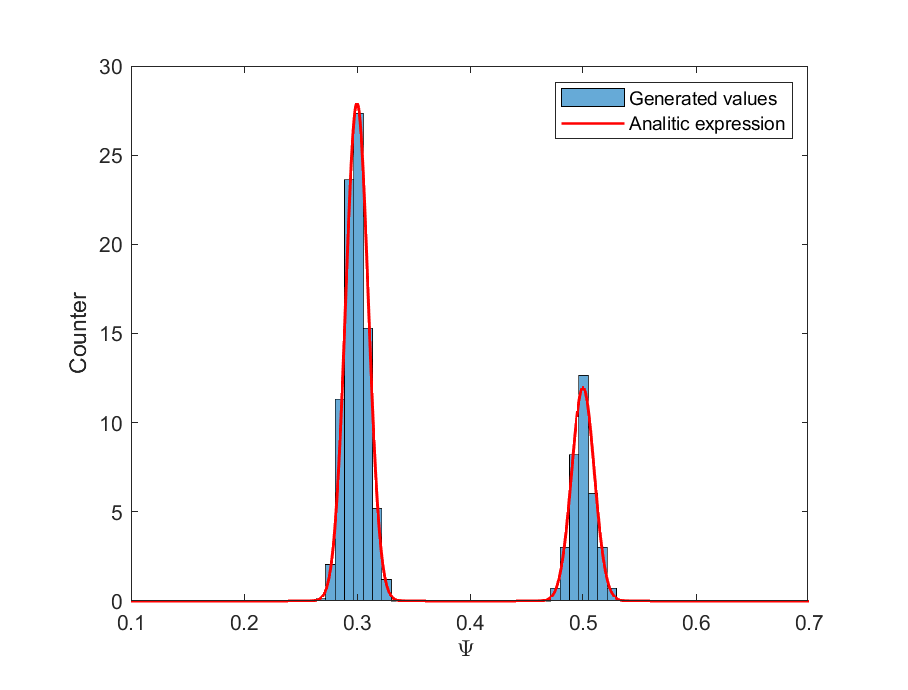
\includegraphics{validation/1paramData.eps}
			\caption{Synthetic data generated sampling a bimodal Gaussian Mixture with peaks at 0.3 and 0.5. The dataset consists in 200 values.}
			\label{val: 1paramData}
		\end{figure}
		
		The synthetic data set is generated starting from an arbitrarily chosen distribution of shape parameters. For simplicity, we will start considering only one parameter, namely $ \psi $. The distribution of $ \psi $ is a bimodal Gaussian Mixture, with the two maxima in $ \underline{\mu} = [0.3, 0.5] $ and a constant standard deviation $ \sigma_{\psi} $ of 0.01. The two modes are chosen with different mixing length: $ \underline{\pi} = [0.7, 0.3] $.
		This distribution can represent a cloud composed at the 70\% of particles with a shape descriptor $ \psi_1 $ of 0.3 and at the 30\% of particles with $ \psi_2 = 0.5 $. The deviation of the data from their nominal value can be associated both with measurement errors, and with the natural dispersion of the particle shapes (that is a characteristic of snowflakes).
		The analytical expression of the distribution $ N(\Psi) $ reads:
		\begin{equation}
			N(\psi) = \dfrac{1}{\sigma_{\Psi} \sqrt{2 \pi}} \ \bigg(
			          e^{-\dfrac{(\psi - \mu_1)^2}{2 \sigma_{\psi}^2}}
			        + e^{-\dfrac{(\psi - \mu_2)^2}{2 \sigma_{\psi}^2}} \bigg) 
		\end{equation}
		
		This formula is sampled 200 times and the discrete distribution is showed in the histogram of \fref{fig: 1paramData}. The generated valued are then used to create an artificial dataset, with each datum described by a volume diameter $ \dv $, a measurement error $ \sigma $, and a terminal velocity $ \vt $, which is calculated using the corresponding value of the shape descriptor $ \psi $. Since we are considering only one parameter, the velocity cannot be calculated with the model of H\"oltzer and Sommerfeld, and the use of an older model which depends only on one shape parameter will be meaningless. Therefore, the velocity is calculated using an arbitrary analytical formula, which, for simplicity, is:
		\begin{equation}
			\vt(\dv, \psi) = \dv \cdot \psi
		\end{equation}
		The same formula will indeed be used to calculate the terminal velocity during the parameter estimation.
		The diameter is also chosen arbitrarily, here random values of about 2-3mm are used.	
		\begin{figure}
			\centering
			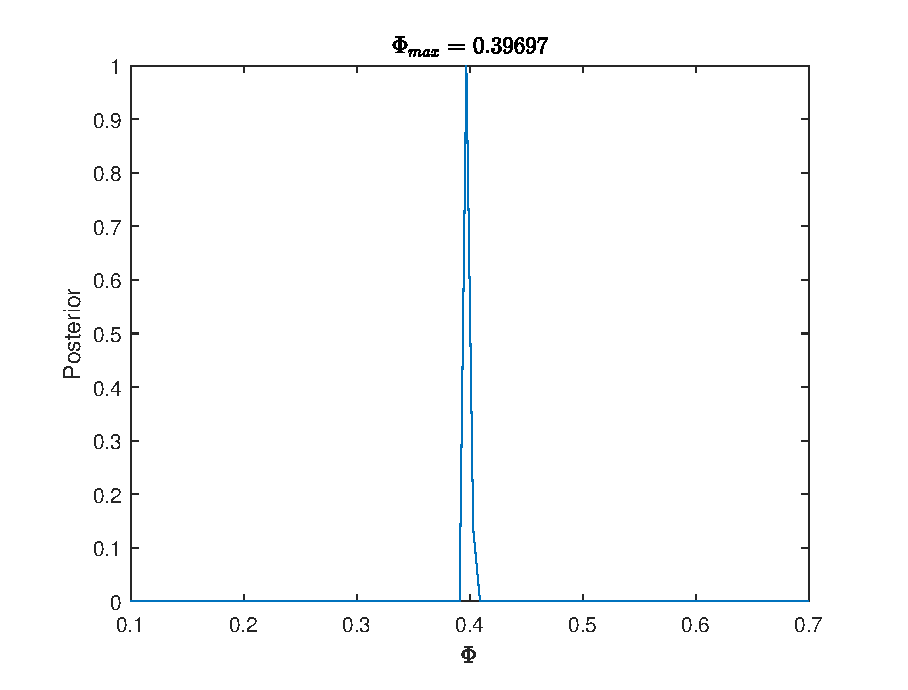
\includegraphics{validation/1param1.eps}
			\caption{}
			\label{val: 1param1}
		\end{figure}
		
		As discussed in \sref{sec: numericalImplementation}, the procedure to infer the parameter distribution is iterative. The first attempt is made allowing one single mode in the posterior (M = 1) and, since the number of parameters involved has been \red{chosen} to be small on purpose, the brute force algorithm is used. In this way the whole posterior is calculated (instead of only its maximum), and it can be graphically represented, as shown in \fref{fig: 1param1}. As expected the posterior has a maximum that is different from both $ \mu_1 $ and $ \mu_2 $. The choice of M = 1 means, as explained in \sref{sec: Bayes} and \ref{sec: GMM}, that the code infers the single, best parameter that explains all the data considered. The calculated maximum $ \psi = 0.35 $ is approximately the weighted average of $ \mu_1 $ and $ \mu_2 $, which is $ 0.7 \mu_1 + 0.3 \mu_2 = 0.36 $.
		
		The procedure requires then to increase the number of modes allowed, thus M is set to 2 and the posterior is computed again. The results are shown in \fref{fig: 1param2}. 
		
		The posterior has two equivalent maxima, in fact the problem is invariant to the transformation described in \eref{eq: transformation}.
		\begin{equation}
			\begin{cases}
				\psi_1 = \psi_2\\
				\psi_2 = \psi_1
			\end{cases}
			\label{eq: transformation}
		\end{equation}
		For the sake of completeness both the posterior are shown and explained this time, but, since the information they provide is the same, from now on, only one maximum per solution will be considered.
		\begin{figure}
			\centering
			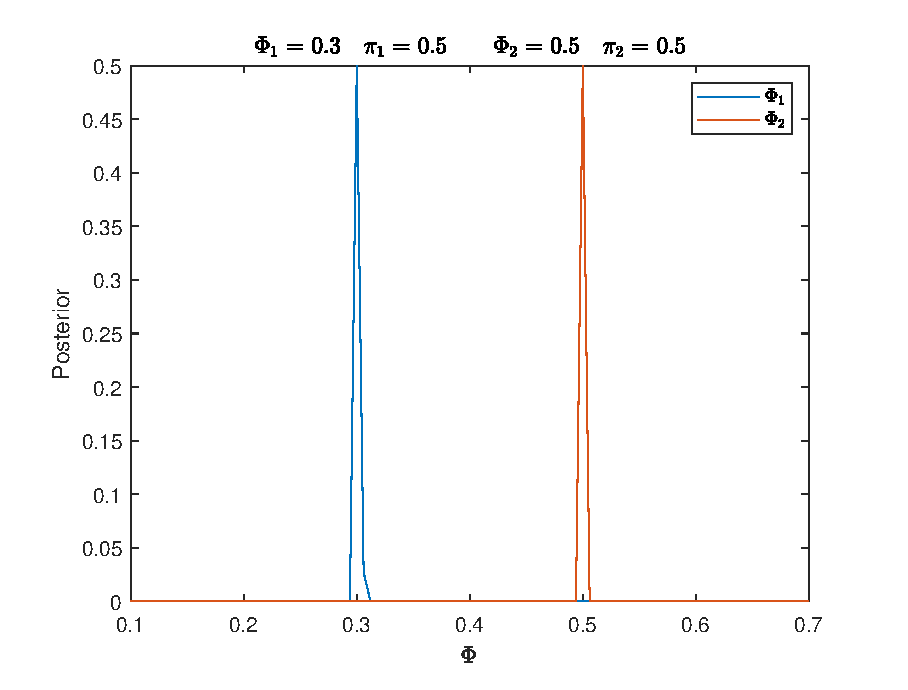
\includegraphics{validation/1param2.eps}
			\caption{}
			\label{val: 1param2}
		\end{figure}
	
		Being M = 2, the posterior has three independent parameters that are inferred: the maximum of the first mode $ \psi_1 $, the maximum of the second mode $ \psi_2 $ and the independent mixing length $ \pi $ (see \sref{sec: GMM}). The two actual values of the mixing length are then reconstructed applying the constraint described in \red{missing reference}, obtaining:
		\begin{equation}
			\begin{cases}
				\pi_1 = \pi \\
				\pi_2 = 1 - \pi
			\end{cases}
			\label{eq: 2ML}
		\end{equation}
		The two modes, which belong to the first maximum (denoted with the superscript 1), are $ (\psi_1, \pi_1)^1 = (0.3, 0.7)  $ and $ (\psi_2, \pi_2)^1 = (0.5, 0.3) $, as written in the title of \fref{fig: 1param2a}. On the figure itself are represented two curves: the first one (blue line) shows the dependency of the posterior on the first mode, with the value of the second mode and the mixing length taken as constants and corresponding to the maximum, namely $ P(\psi_1) = P(\psi_1, \psi_{2, \textup{max}}, \pi_{\textup{max}}) $; the second one (red line) shows the same dependency w.r.t the second mode: $ P(\psi_2) = P(\psi_{1, \textup{max}}, \psi_2, \pi_{\textup{max}}) $.
		Following the same scheme, \fref{fig: 1param2b} shows that the second maximum contains the two modes  $ (\psi_1, \pi_1)^2 = (0.5, 0.3)  $ and $ (\psi_2, \pi_2)^2 = (0.3, 0.7) $.
		These are indeed the results that we were looking for, but the procedure now provides that the number of modes is increased again, and only if the solution at M = 3 coincides with the previous one (M = 2) we can exit the loop. 
		
		The posterior resulting from the third iteration of the scheme is represented in \fref{1param3}. \red{instert comment}
		\begin{figure}
			\centering
			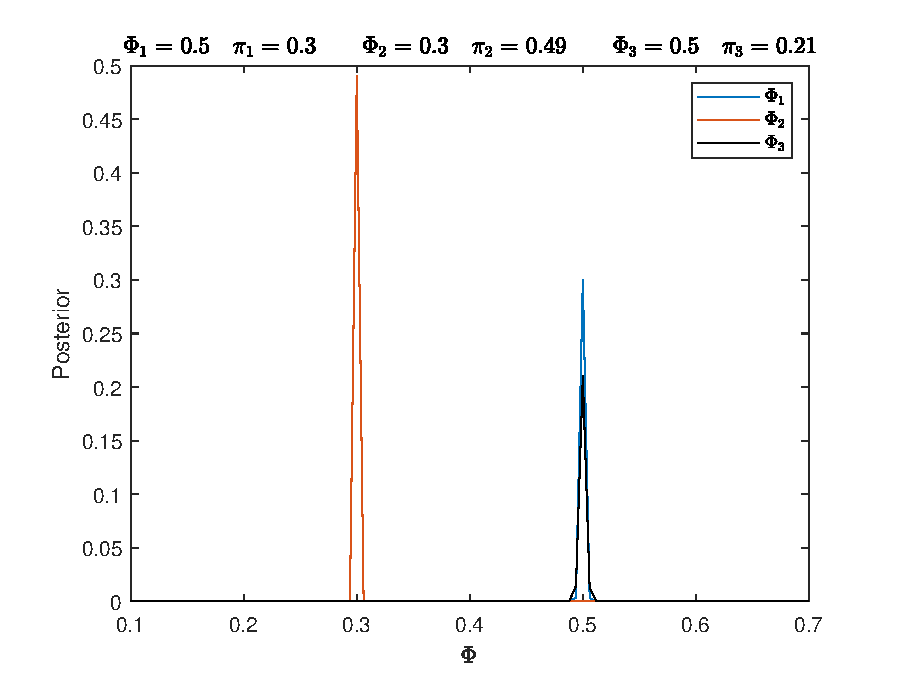
\includegraphics{validation/1param3.eps}
			\caption{}
			\label{val: 1param3}
		\end{figure}
		
		
		
		
		
		
		
		
		
		
		
		
		
		
		
		
		
		
		
		
		
		\begin{itemize}
			\item 1 parameter (\fref{val: 1paramData}, \ref{val: 1param1}, \ref{val: 1param2}, \ref{val: 1param3})
			\item 2 parameters (\fref{val: 2paramData}, \ref{val: 2param1}, \ref{val: 2param2})
		\end{itemize}
	
		

		\begin{figure}
			\centering
			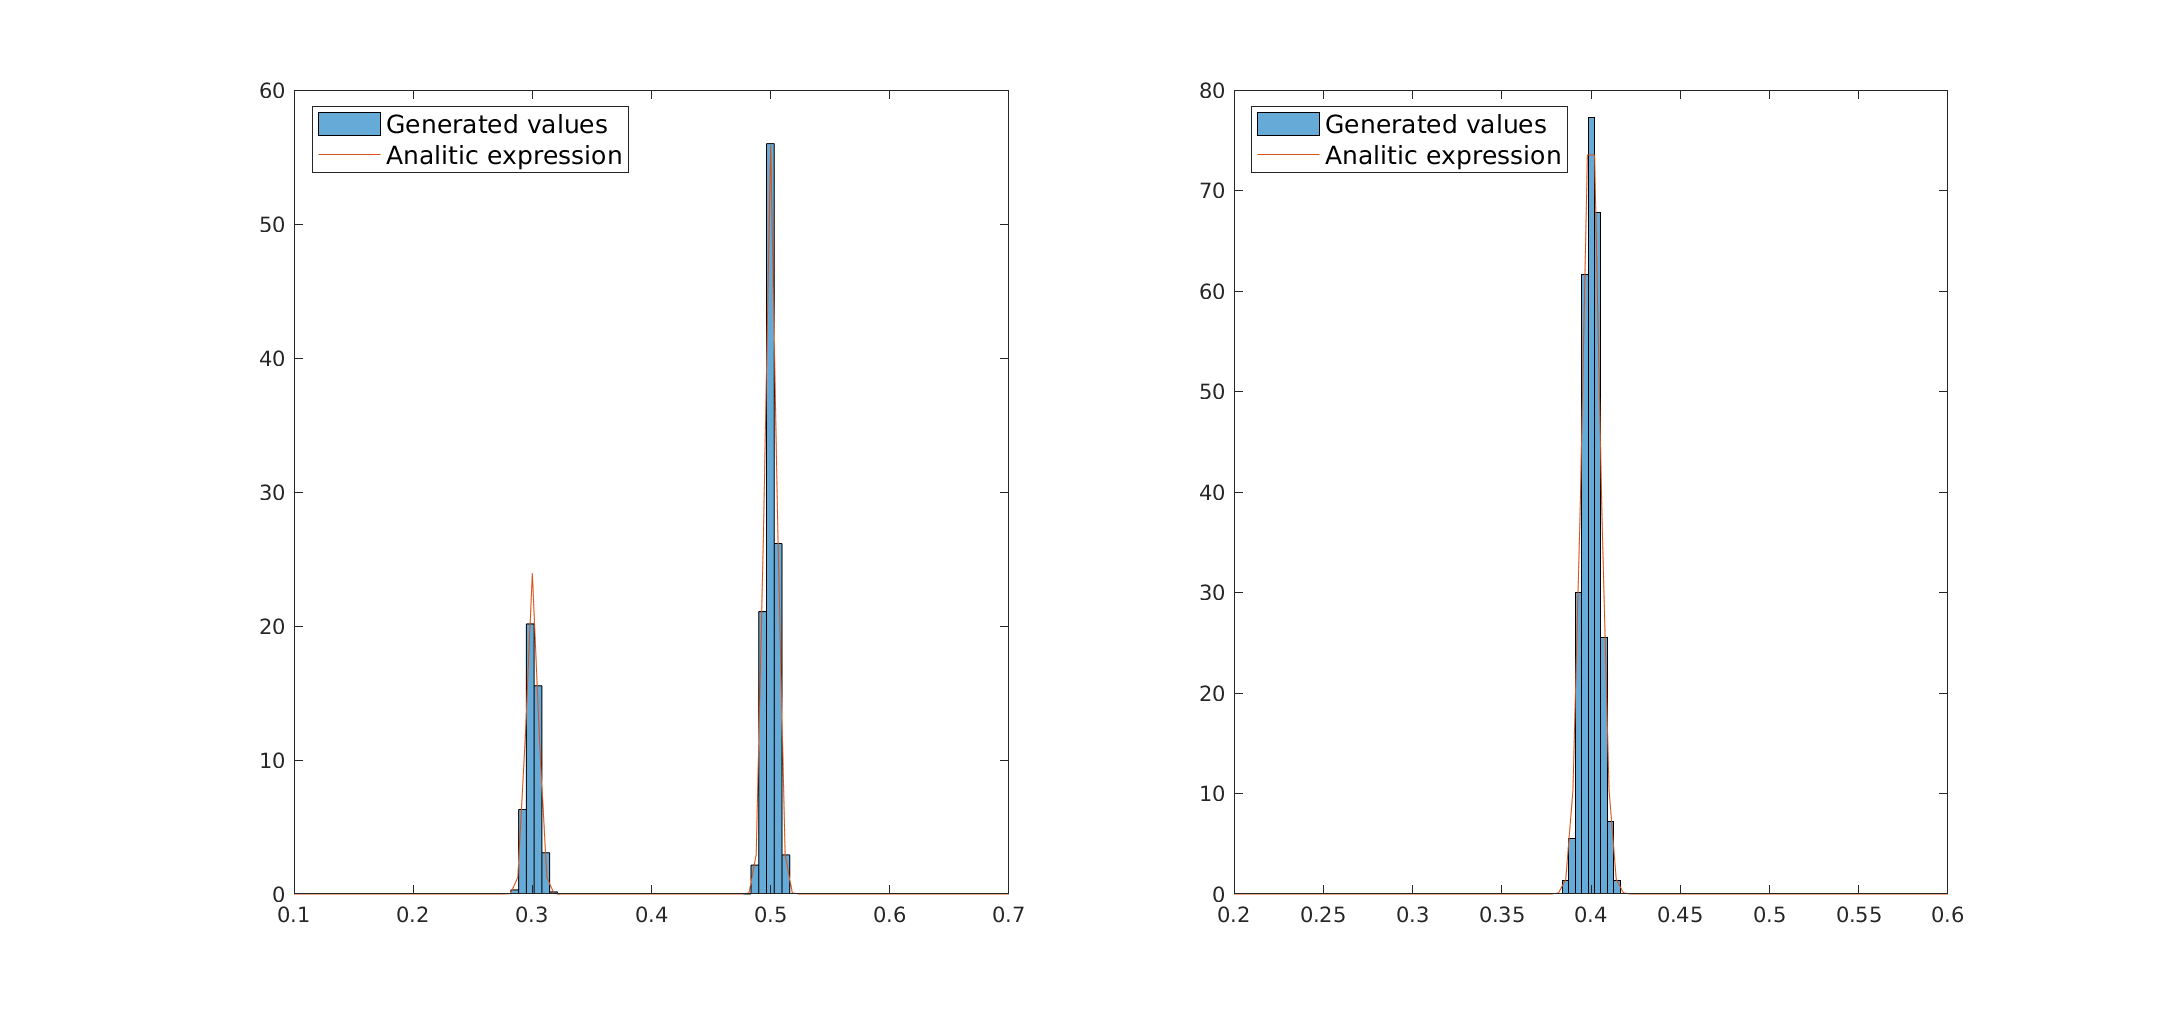
\includegraphics[width=\linewidth]{validation/2paramData.eps}
			\caption{}
			\label{val: 2paramData}
		\end{figure}
		\begin{figure}
			\centering
			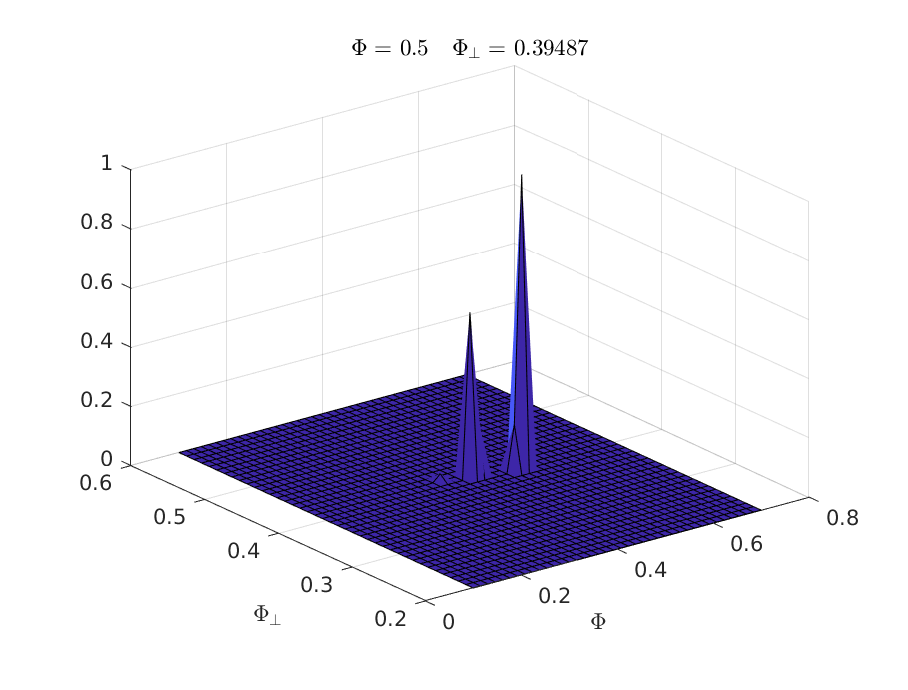
\includegraphics[width=\linewidth]{validation/2param1.eps}
			\caption{}
			\label{val: 2param1}
		\end{figure}
		\begin{figure}
			\centering
			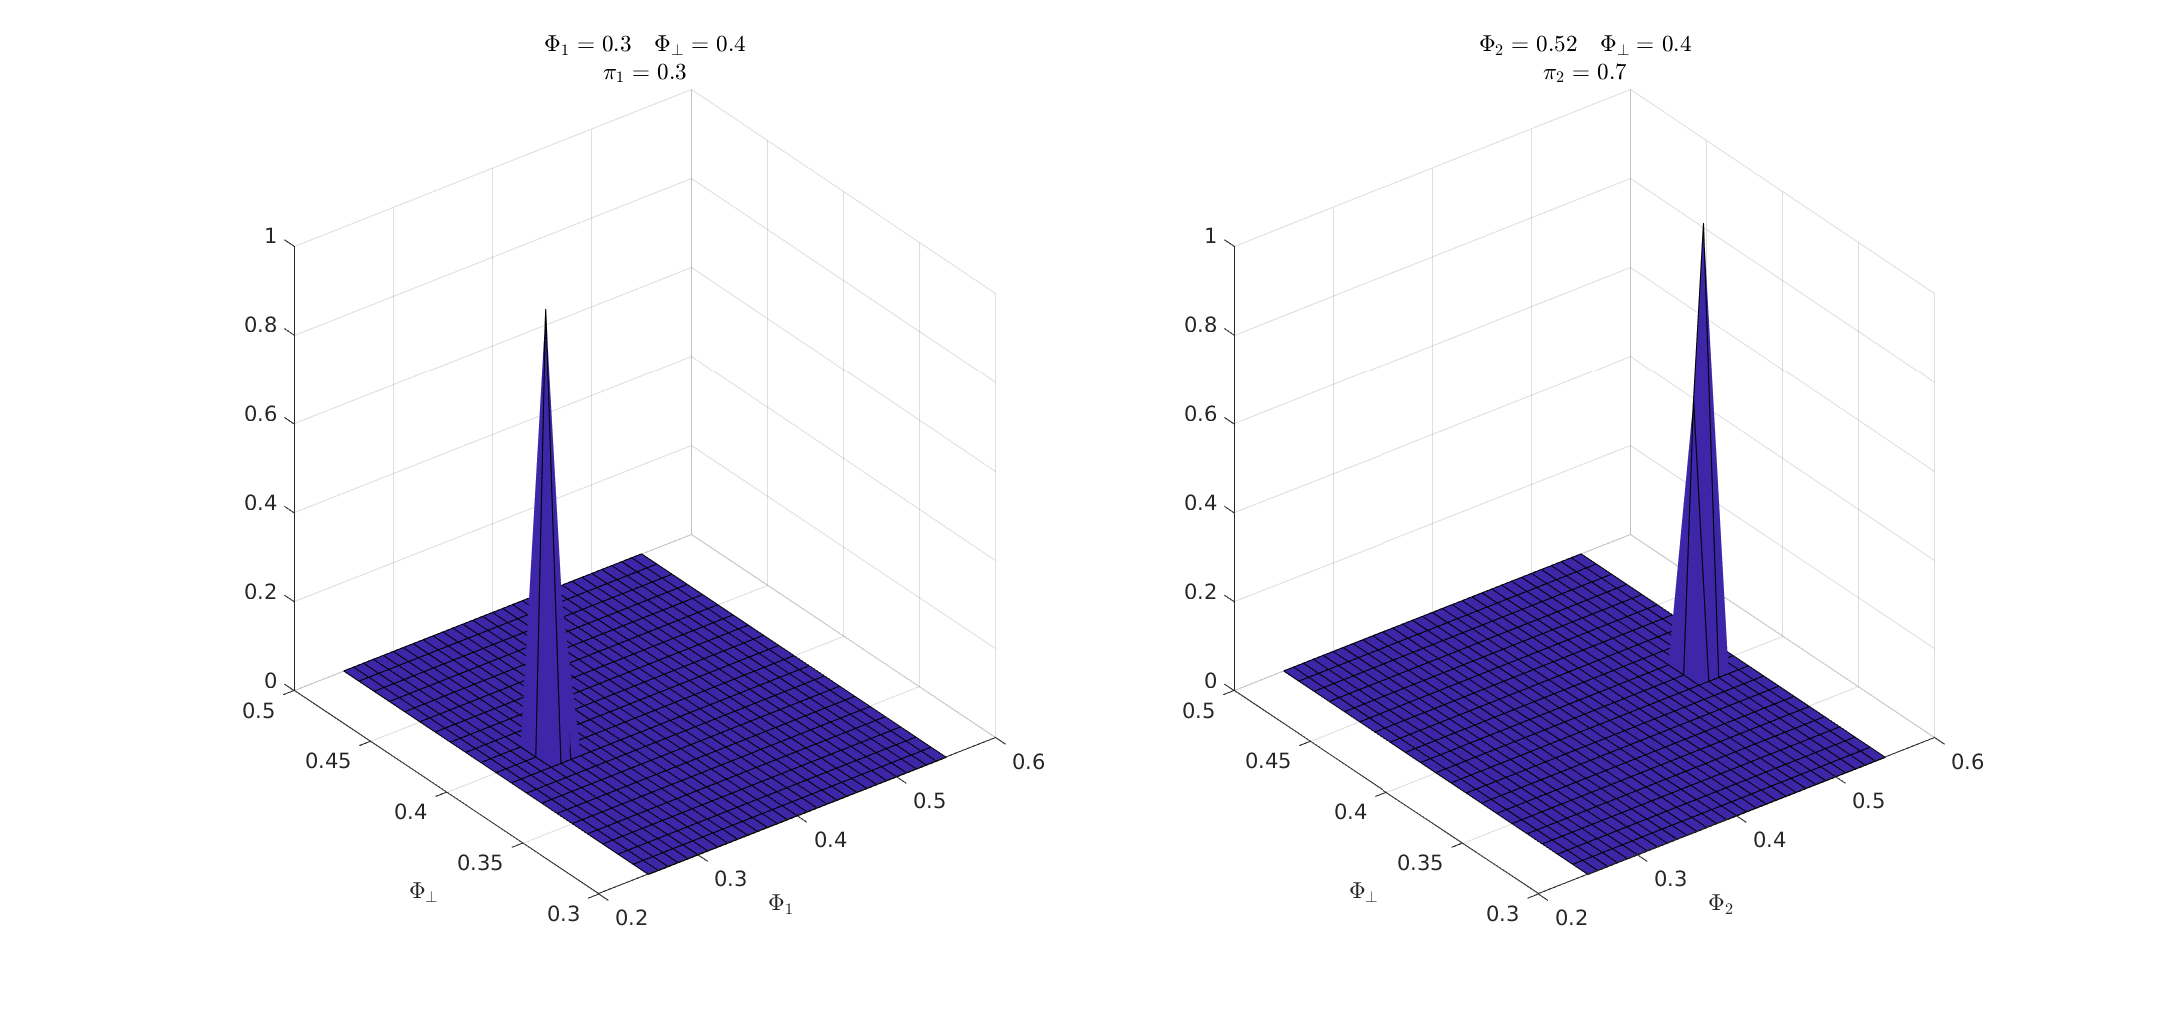
\includegraphics[width=\linewidth]{validation/2param2.eps}
			\caption{}
			\label{val: 2param2}
		\end{figure}

	\section{Test case 2 - Experimental Dataset}
	\label{sec: TC2}
		Brief description of the available experimental campaigns (Brandes + other 2 references) and their limitations.
	
		\subsection{Brandes Experimental campaign}
		\label{sec: BrandesExp}
		Description of the Brandes results and impossibility to use the raw data
		
		\subsection{Data Set generation}
		\label{sec: dataGeneration}
		Generation of an artificial data set starting from the relations discovered by Brandes. The dependency on the diameter distribution is not taken into account as it can be retrieved a posteriori.
	
		\subsection{Application to the Brandes data set}
		\label{sec: results}
		\begin{itemize}
			\item Example for 1 diameter interval
			\item Shape parameters - diameter distribution (Work in progress)
		\end{itemize}
		
	\section{Test case 3 - Let it snow!}
		Falling snow test case (Check the terminal velocity distribution) with PoliDrop
